% Options for packages loaded elsewhere
\PassOptionsToPackage{unicode}{hyperref}
\PassOptionsToPackage{hyphens}{url}
%
\documentclass[
]{article}
\usepackage{amsmath,amssymb}
\usepackage{lmodern}
\usepackage{iftex}
\ifPDFTeX
  \usepackage[T1]{fontenc}
  \usepackage[utf8]{inputenc}
  \usepackage{textcomp} % provide euro and other symbols
\else % if luatex or xetex
  \usepackage{unicode-math}
  \defaultfontfeatures{Scale=MatchLowercase}
  \defaultfontfeatures[\rmfamily]{Ligatures=TeX,Scale=1}
\fi
% Use upquote if available, for straight quotes in verbatim environments
\IfFileExists{upquote.sty}{\usepackage{upquote}}{}
\IfFileExists{microtype.sty}{% use microtype if available
  \usepackage[]{microtype}
  \UseMicrotypeSet[protrusion]{basicmath} % disable protrusion for tt fonts
}{}
\makeatletter
\@ifundefined{KOMAClassName}{% if non-KOMA class
  \IfFileExists{parskip.sty}{%
    \usepackage{parskip}
  }{% else
    \setlength{\parindent}{0pt}
    \setlength{\parskip}{6pt plus 2pt minus 1pt}}
}{% if KOMA class
  \KOMAoptions{parskip=half}}
\makeatother
\usepackage{xcolor}
\usepackage[margin=1in]{geometry}
\usepackage{longtable,booktabs,array}
\usepackage{calc} % for calculating minipage widths
% Correct order of tables after \paragraph or \subparagraph
\usepackage{etoolbox}
\makeatletter
\patchcmd\longtable{\par}{\if@noskipsec\mbox{}\fi\par}{}{}
\makeatother
% Allow footnotes in longtable head/foot
\IfFileExists{footnotehyper.sty}{\usepackage{footnotehyper}}{\usepackage{footnote}}
\makesavenoteenv{longtable}
\usepackage{graphicx}
\makeatletter
\def\maxwidth{\ifdim\Gin@nat@width>\linewidth\linewidth\else\Gin@nat@width\fi}
\def\maxheight{\ifdim\Gin@nat@height>\textheight\textheight\else\Gin@nat@height\fi}
\makeatother
% Scale images if necessary, so that they will not overflow the page
% margins by default, and it is still possible to overwrite the defaults
% using explicit options in \includegraphics[width, height, ...]{}
\setkeys{Gin}{width=\maxwidth,height=\maxheight,keepaspectratio}
% Set default figure placement to htbp
\makeatletter
\def\fps@figure{htbp}
\makeatother
\setlength{\emergencystretch}{3em} % prevent overfull lines
\providecommand{\tightlist}{%
  \setlength{\itemsep}{0pt}\setlength{\parskip}{0pt}}
\setcounter{secnumdepth}{5}
\newlength{\cslhangindent}
\setlength{\cslhangindent}{1.5em}
\newlength{\csllabelwidth}
\setlength{\csllabelwidth}{3em}
\newlength{\cslentryspacingunit} % times entry-spacing
\setlength{\cslentryspacingunit}{\parskip}
\newenvironment{CSLReferences}[2] % #1 hanging-ident, #2 entry spacing
 {% don't indent paragraphs
  \setlength{\parindent}{0pt}
  % turn on hanging indent if param 1 is 1
  \ifodd #1
  \let\oldpar\par
  \def\par{\hangindent=\cslhangindent\oldpar}
  \fi
  % set entry spacing
  \setlength{\parskip}{#2\cslentryspacingunit}
 }%
 {}
\usepackage{calc}
\newcommand{\CSLBlock}[1]{#1\hfill\break}
\newcommand{\CSLLeftMargin}[1]{\parbox[t]{\csllabelwidth}{#1}}
\newcommand{\CSLRightInline}[1]{\parbox[t]{\linewidth - \csllabelwidth}{#1}\break}
\newcommand{\CSLIndent}[1]{\hspace{\cslhangindent}#1}
\usepackage{setspace}\onehalfspacing
\usepackage{float}
\usepackage{caption}
\captionsetup[figure]{labelformat=empty}
\usepackage{booktabs}
\usepackage{longtable}
\usepackage{array}
\usepackage{multirow}
\usepackage{wrapfig}
\usepackage{float}
\usepackage{colortbl}
\usepackage{pdflscape}
\usepackage{tabu}
\usepackage{threeparttable}
\usepackage{threeparttablex}
\usepackage[normalem]{ulem}
\usepackage{makecell}
\usepackage{xcolor}
\ifLuaTeX
  \usepackage{selnolig}  % disable illegal ligatures
\fi
\IfFileExists{bookmark.sty}{\usepackage{bookmark}}{\usepackage{hyperref}}
\IfFileExists{xurl.sty}{\usepackage{xurl}}{} % add URL line breaks if available
\urlstyle{same} % disable monospaced font for URLs
\hypersetup{
  pdftitle={Bluefin Combined Index Model V1},
  pdfauthor={Katie Lankowicz},
  hidelinks,
  pdfcreator={LaTeX via pandoc}}

\title{Bluefin Combined Index Model V1}
\author{Katie Lankowicz}
\date{30 June, 2023}

\begin{document}
\maketitle

{
\setcounter{tocdepth}{2}
\tableofcontents
}
\hypertarget{motivation}{%
\section{Motivation}\label{motivation}}

In the last several decades, global climate change has resulted in warming ocean temperatures and altered marine habitat suitability. Responses to these environmental changes can be seen at the individual, population, and ecosystem level for many marine fish species. Frequently, marine fish will shift their spatial-temporal distribution to track environmental conditions that are better-suited to their energetic requirements. It is suspected that the western stock of Atlantic Bluefin Tuna (BFT) is currently undergoing a climate-forced range shift due to rapidly warming conditions in the Northwest Atlantic. Recent stock assessments for BFT in US and Canadian waters have provided conflicting trends in catch-per-unit-effort (CPUE) indices for BFT, where the Canadian fishery has seen an increase in BFT CPUE and the American fishery has seen a decrease.

This project will create a joint CPUE index for BFT across American and Canadian waters in the Northwest Atlantic using Vector Autoregressive Spatio-Temporal (VAST) modeling. VAST is a flexible model framework based on delta-generalized linear mixed models, and is capable of incorporating information from multiple sources and gear types to create a joint index. VAST can also incorporate the effects of habitat and catchability covariates on organism spatio-temporal distribution. VAST outputs include spatial metrics including spatio-temporal density maps, hierarchical clustering of spatial areas based on organism density, stock center of gravity, area of utilization, and quantile of range edges.

The remainder of this document will be used to report progress on cleaning and merging American and Canadian BFT catch data and making VAST model structure decisions.

\hypertarget{bft-data}{%
\section{BFT data}\label{bft-data}}

BFT data from American and Canadian fisheries are in variable formats and need to be heavily manipulated prior to merging. The goal is to create a dataframe where each row represents a sampling event. The following variables are desired for each sampling event:

\begin{itemize}
\tightlist
\item
  Unique trip identifier
\item
  Date
\item
  Spatial location (latitude and longitude, decimal degrees)
\item
  Number of hours spent fishing
\item
  Number of BFT caught in both large and small size groups
\item
  Sea surface temperature
\item
  Water depth
\item
  Sea level pressure
\item
  Basin-wide daily NAO index
\item
  Basin-wide monthly AMO index
\item
  Wind direction and velocity
\item
  Local chlorophyll-A concentration (as a proxy for plankton distribution)
\item
  Local prey biomass
\end{itemize}

\hypertarget{model-domains}{%
\subsection{Model domains}\label{model-domains}}

Currently, the model's temporal domain is 1993 - 2020. Though BFT total catch data were recorded prior to 1993, information to determine the size of each fish was not reliably recorded. The final model will include indices for multiple BFT size classes, and so data without associated length or weight information is not useful. The temporal domain currently ends at 2020 because that is the most recent year with Canadian catch data. American catch data ends at 2021. The temporal domain could be extended with new information.

The model spatial domain is the combined area of American and Canadian exclusive economic zones (EEZs) in the Northwest Atlantic, bounded on the south by Cape Hatteras, North Carolina and on the north by Cape North, Nova Scotia. The model does not consider the Gulf of Saint Lawrence, nor is any tuna catch data from that area included. The model will estimate indices of abundance within both of the spatial strata-- US EEZ waters and Canadian EEZ waters.

\begin{verbatim}
## Reading layer `NWAtlantic' from data source 
##   `C:\Users\klankowicz\Documents\GitHub\Atlantic-Bluefin-Tuna-Climate-Informed-Stock-Assessment\Data\GIS\NWAtlantic.shp' 
##   using driver `ESRI Shapefile'
## Simple feature collection with 1 feature and 1 field
## Geometry type: POLYGON
## Dimension:     XY
## Bounding box:  xmin: -8460792 ymin: 4196772 xmax: -7313632 ymax: 5648546
## Projected CRS: WGS 84 / Pseudo-Mercator
\end{verbatim}

\begin{verbatim}
## Reading layer `CanadaEEZ' from data source 
##   `C:\Users\klankowicz\Documents\GitHub\Atlantic-Bluefin-Tuna-Climate-Informed-Stock-Assessment\Data\GIS\CanadaEEZ.shp' 
##   using driver `ESRI Shapefile'
## Simple feature collection with 1 feature and 4 fields
## Geometry type: POLYGON
## Dimension:     XY
## Bounding box:  xmin: -7541061 ymin: 4871320 xmax: -6131963 ymax: 5909353
## Projected CRS: WGS 84 / Pseudo-Mercator
\end{verbatim}

\begin{figure}
\centering
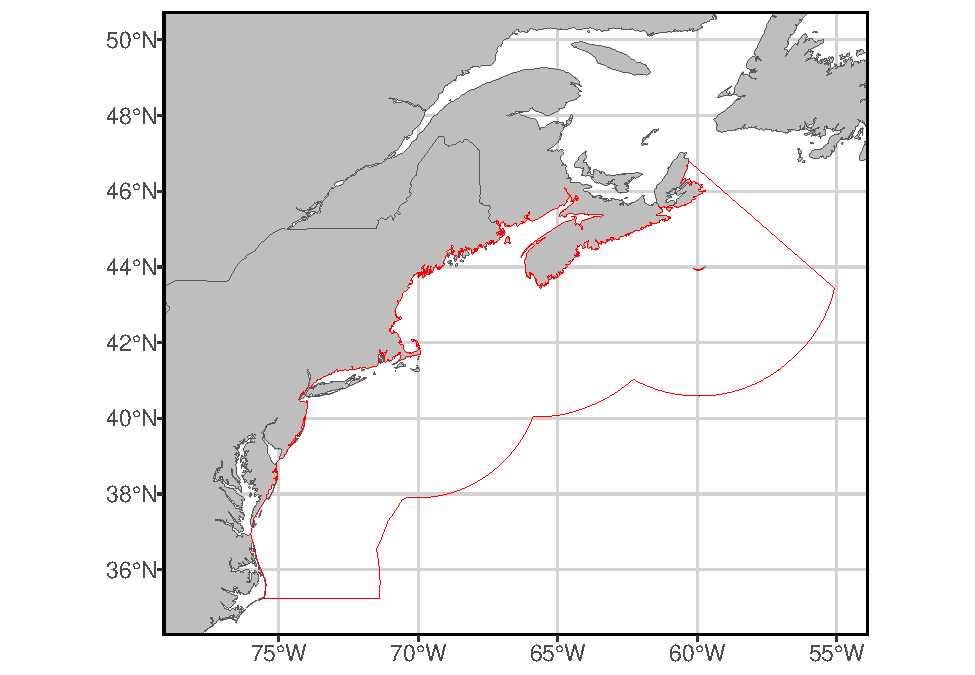
\includegraphics{Model_Prelim_Report_files/figure-latex/spatial-domain-1.pdf}
\caption{\label{fig:spatial-domain}Fig. 1: VAST model spatial domain}
\end{figure}

\hypertarget{bft-size-categories}{%
\subsection{BFT size categories}\label{bft-size-categories}}

BFT are categorized into six size classes by both weight and length. BFT migrations and habitat use are expected to vary with age, and so the ideal model will generate separate indices and spatial metrics for different age groupings. There is not enough information to do this for each of the six size classes, and so the size class information was pooled into two groupings: small and large. Small BFT are 144 cm (56.7 in) and shorter, while large BFT are longer than 177 cm (69.7 in). This structure was chosen to match the structure of current US handline BFT indices. Because the ``Small medium'' size class straddles the line between groups, these fish have been excluded from analysis.

BFT were categorized according to length, preferentially. If no length information was recorded, weight was used to categorize. If neither length nor weight information was recorded for a fish, it could not be included in analysis.

\begin{table}[H]

\caption{\label{tab:size-table}Bluefin tuna size classes}
\centering
\begin{tabular}[t]{lllll}
\toprule
Size class & Grouping & Curved Fork
Length & Pectoral Curved
Fork Length & Weight (lbs)\\
\midrule
Young school & Small & <27 in & <20 in & <14 lbs\\
School & Small & 27 - <47 in & 20 - <35 in & 14 - <66 lbs\\
Large school & Small & 47 - <59 in & 35 - <44 in & 66 - <135 lbs\\
Small medium & NA & 59 - <73 in & 44 - <54 in & 135 - <235 lbs\\
Large medium & Large & 73 - <81 in & 54 - <60 in & 235 - <310 lbs\\
\addlinespace
Giant & Large & 81+ in & 60+ in & 310+ lbs\\
\bottomrule
\end{tabular}
\end{table}

\hypertarget{environmental-covariates}{%
\subsection{Environmental covariates}\label{environmental-covariates}}

Several ocean climate variables and static properties are expected to cause shifts in BFT distribution. For this model, we will include sea surface temperature, sea level pressure, basin-wide daily NAO, basin-wide monthly AMO, and water depth. When building the VAST model, these will be called density covariates.

\hypertarget{us-bft-recreational-catch}{%
\subsection{US BFT Recreational Catch}\label{us-bft-recreational-catch}}

Catch and effort information for the US recreational BFT fishery is recorded by the Large Pelagics Survey, which is a dockside/telephone survey of a random sample of private and charter boat captains targeting large pelagics. We subset the full LPS dataset so only data from trips targeting BFT were included. Other filters were also applied: only tuna landed in Virginia and northwards were included, fishing trips needed to be between 1 and 24 hours in length, and only fishing trips ending on June 1st through October 31st of each year were included.

LPS data recording procedures changed in 2002, and so data are stored across two sets of files (1993-2002, 2002-present). These needed to be cleaned and merged. This process can be viewed in the accompanying RMarkdown document. An example of results will also be provided.

Note that sea surface temperature and water depth are not always provided by the anglers. We have merged these spatiotemporal catch data with NOAA 1/4° Daily Optimum Interpolation Sea Surface Temperature (OISST) and GEBCO 15 arc-second gridded bathymetric data to get complete data coverage for SST and depth.

\begin{landscape}\begin{table}[H]

\caption{\label{tab:mergelps}American Large Pelagic Survey example}
\centering
\begin{tabular}[t]{lrrrrrrrrrrrrr}
\toprule
Size & Trip
ID & Year & Month & Day & Hours
fished & Lon & Lat & nCatch & SST
(C) & Depth
(m) & Pressure & NAO & AMO\\
\midrule
large & 2 & 1993 & 10 & 1 & 6 & -71.36667 & 40.03333 & 0 & 19.65 & -6.7 & 102403 & 0.7010462 & -0.259\\
small & 3 & 1993 & 10 & 1 & 6 & -71.36667 & 40.03333 & 1 & 19.65 & -6.7 & 102403 & 0.7010462 & -0.259\\
large & 3 & 1993 & 10 & 1 & 6 & -71.36667 & 40.03333 & 0 & 19.65 & -6.7 & 102403 & 0.7010462 & -0.259\\
small & 2 & 1993 & 10 & 1 & 6 & -71.36667 & 40.03333 & 2 & 19.65 & -6.7 & 102403 & 0.7010462 & -0.259\\
large & 1 & 1993 & 10 & 2 & 9 & -70.50000 & 42.16667 & 0 & 13.62 & -5.2 & 101980 & 0.9867340 & -0.259\\
\addlinespace
small & 1 & 1993 & 10 & 2 & 9 & -70.50000 & 42.16667 & 10 & 13.62 & -5.2 & 101980 & 0.9867340 & -0.259\\
\bottomrule
\end{tabular}
\end{table}
\end{landscape}

\begin{figure}
\centering
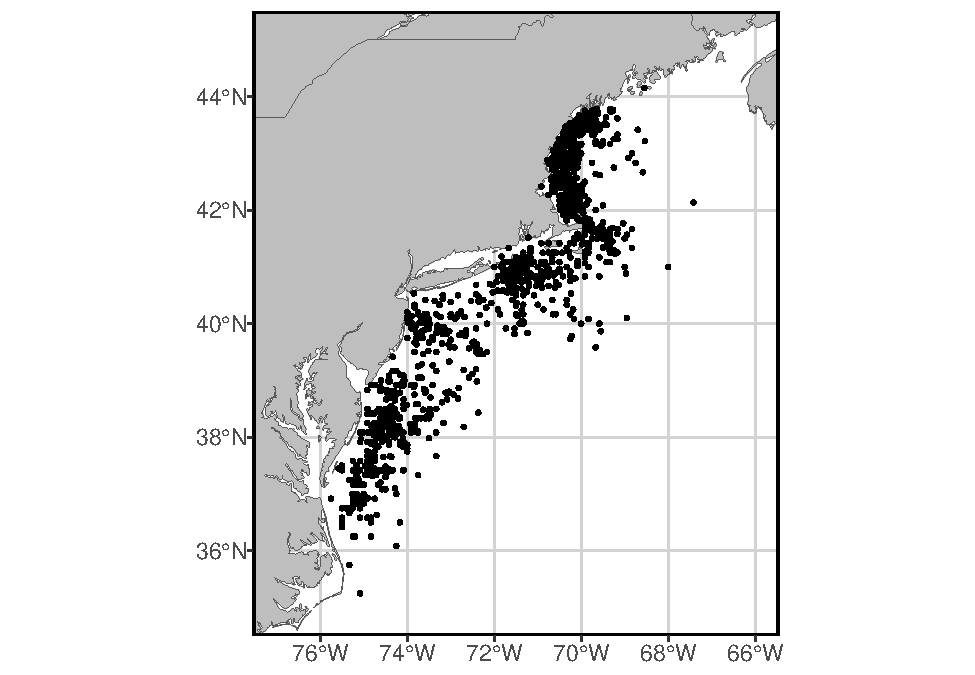
\includegraphics{Model_Prelim_Report_files/figure-latex/americanplot-1.pdf}
\caption{\label{fig:americanplot}Fig. 2: Spatial distribution of American recreational catch}
\end{figure}

\hypertarget{canadian-bft-commercial-landings}{%
\subsection{Canadian BFT Commercial Landings}\label{canadian-bft-commercial-landings}}

Catch and effort data for the Canadian commercial BFT fishery are recorded in commercial logbooks. We will only be working with commercial data from the Southwest Nova Scotia region, though data exists for the Gulf of Saint Lawrence region as well. The same data filters regarding fishing hours and month fished applied to the US data were applied to the Canadian data. Though the US recreational fishery is likely all rod and reel, the Canadian commercial fishery also includes harpoon and tended line gear. This could later inform some model structure decisions.

Data collection methods changed in 2003, and so the data are stored across two sets of files (Commercial Landings 95-03, Historical Data. These needed to be cleaned and merged. This process can be viewed in the accompanying RMarkdown document. An example of results will also be provided.

There are some concerns with the historic (1993-2002) Canadian data. The data have several columns that I cannot make sense of without metadata. Although I assume I have only been provided with BFT catch, there is a column for species landed in the data. The values within this column are numeric (252-256), and I do not know what these numbers mean. For now, I have made the assumption that all these species codes refer to BFT. In the future, I can subset out non-BFT data if I am made aware that some of these species codes are not BFT.

\begin{landscape}\begin{table}[H]

\caption{\label{tab:mergecan}Canadian commercial data example}
\centering
\begin{tabular}[t]{lrrrrrrrrrrrrr}
\toprule
Size & Trip
ID & Year & Month & Day & Hours
fished & nCatch & SST
(C) & Depth
(m) & Pressure & NAO & AMO & Lon & Lat\\
\midrule
large & 1 & 1993 & 10 & 1 & 8 & 0 & 15.42 & -165.0 & 102205 & 0.7010462 & -0.259 & -65.21667 & 42.96667\\
Unknown & 1 & 1993 & 10 & 1 & 8 & 10 & 15.42 & -165.0 & 102205 & 0.7010462 & -0.259 & -65.21667 & 42.96667\\
small & 1 & 1993 & 10 & 1 & 8 & 0 & 15.42 & -165.0 & 102205 & 0.7010462 & -0.259 & -65.21667 & 42.96667\\
small & 2 & 1993 & 10 & 2 & 8 & 0 & 15.77 & -378.1 & 102585 & 0.9867340 & -0.259 & -65.60000 & 42.05000\\
large & 2 & 1993 & 10 & 2 & 8 & 0 & 15.77 & -378.1 & 102585 & 0.9867340 & -0.259 & -65.60000 & 42.05000\\
\addlinespace
Unknown & 2 & 1993 & 10 & 2 & 8 & 2 & 15.77 & -378.1 & 102585 & 0.9867340 & -0.259 & -65.60000 & 42.05000\\
\bottomrule
\end{tabular}
\end{table}
\end{landscape}

\begin{figure}
\centering
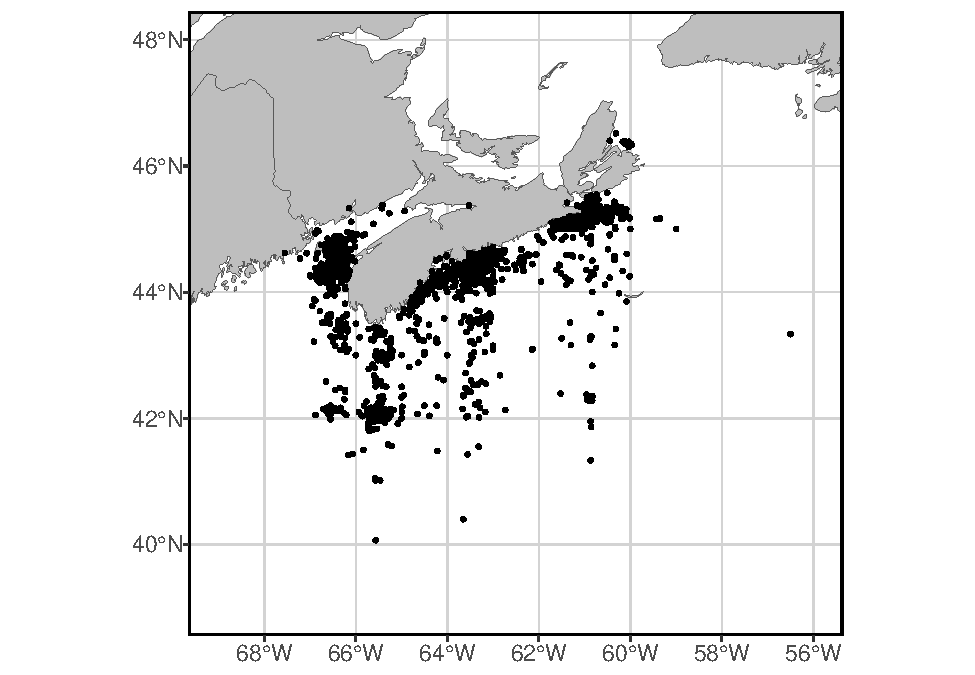
\includegraphics{Model_Prelim_Report_files/figure-latex/canadianplot-1.pdf}
\caption{\label{fig:canadianplot}Fig. 3: Spatial distribution of Canadian commercial catch}
\end{figure}

\hypertarget{data-needs}{%
\subsection{Data needs}\label{data-needs}}

There are a few environmental variables that have not yet been incorporated into the resulting data. I have created a VAST model of prey distribution based on NOAA herring, menhaden, and mackerel observer data. However, these data do not have 0 values (an important part of a VAST model) and do not have any coverage in Canadian waters. It would be best to fill out the data from other sources to get better models of prey spatiotemporal density.

Chloropyll was noted as a potential covariate for BFT distribution, but I have not yet found a data source that has complete coverage in our spatial and temporal domains. VAST models cannot tolerate missing values for density covariates, and the many gaps in MODIS data caused by cloud coverage are currently preventing me from including chlorophyll data. Suggestions are welcomed.

Wind direction and velocity have not yet been incorporated. Ideally, we would have information on the wind direction and velocity at the exact space and time of each tuna observation, though I could extract this information from data with larger spatial grain. I have spent less time looking for a source for these data. Suggestions are welcomed.

\hypertarget{vast}{%
\section{VAST}\label{vast}}

VAST models were used to estimate BFT spatial density over time and create joint indices of abundance using all available American and Canadian catch data. VAST is a framework for implementing spatial delta-generalized linear mixed models (delta-GLMM) and can be manipulated to provide estimates for multiple categories of interest and spatial strata Thorson (\protect\hyperlink{ref-thorson_2019}{2019}). It is structured to utilize two linear predictors; the first linear predictor estimates encounter probability, and the second linear predictor estimates catch rates. The first linear predictor can be represented as

\[\rho_1(i) = \beta_1(c_i, t_i) + \omega_1^*(s_i, c_i) + \varepsilon_1^*(s_i, c_i, t_i) + \eta_1(v_i, c_i) + \nu_1(c_i, t_i)\]

where \(\rho_1(i)\) is the predictor for observation \emph{i} for category \(c_i\) at location \(s_i\) and time \(t_i\). \(\beta_1(c_i, t_i)\) represents temporal variation for each category and time, \(\omega_i(s_i, c_i)\) represents spatial variation for each location and category, \(\varepsilon_1(s_i, c_i, t_i)\) represents spatiotemporal variation for each location, category, and time, \(\eta_1(v_i, c_i)\) represents vessel effects for each vessel and category, and \(\nu_1(c_i, t_i)\) represents the effect of density covariates for each category and time. The second linear predictor is structured the same way. Both linear predictors incorporate fixed and random effects, and spatial and spatiotemporal variation are approximated as Gaussian Markov random fields Thorson (\protect\hyperlink{ref-thorson_2019}{2019}).

Implementation of VAST models requires several structural and data inclusion decisions, as outlined in Thorson (\protect\hyperlink{ref-thorson_2019}{2019}). Decisions used in this effort will be discussed in the following subsections.

\hypertarget{response-variable-and-effort-adjustment}{%
\subsection{Response variable and effort adjustment}\label{response-variable-and-effort-adjustment}}

Our data provide information on the number of fish of each size group caught during each fishing trip, as well as the number of hours fished on that trip. Gear type varies and this likely affects catchability and actual effort. For now, catch will be adjusted for effort by dividing the catch by number of hours fished.

VAST models require an input for effort to scale the response variable. For most fishery-independent surveys, this input would be similar to area swept. For this fishery-dependent dataset utilizing multiple gears, we have already accounted for effort in our manipulation of the response variable. Therefore, we will assign effor to be a unitless 1 for all observations.

\hypertarget{density-and-catchability-covariates}{%
\subsection{Density and Catchability Covariates}\label{density-and-catchability-covariates}}

VAST allows for the effects of both density and catchability covariates to be included in modeling efforts. Catchability covariates are processes one would expect to affect the ability to observe the target organism without necessarily affecting the distribution of the organism. Density covariates are processes that directly affect the distribution of the target organism, regardless of ability to observe it. Both covariates affect the catch rate of the target organism, but only density covariates are used to predict target organism density within the spatial domain. Therefore, VAST ``controls for'' catchability covariates and ``conditions on'' density covariates. VAST is unable to distinguish whether potential covariates should be treated as catchability or density covariates; this must be decided with theoretical insight from an analyst.

In this model, we will utilize the environmental covariates and basin-scale climate indices as density covariates. Density covariates were chosen after a model selection process to determine their utility to describe patterns in BFT spatiotemporal density. Currently, a simple linear model is used to describe the effects of these covariates on BFT CPUE. In the future, other models will be tested; it is likely that the best model will be more fluid, like a generalized additive model using polynomial splines.

We will not explicitly include catchability covariates, but wil allow for variation in catchability between the American and Canadian fisheries by including them as ``vessel effects.''

\hypertarget{error-structure}{%
\subsection{Error structure}\label{error-structure}}

As recommended by model developers for adjusted-effort models, a delta-lognormal distribution was chosen for the first linear predictor and an alternative ``Poisson-link delta-model''was chosen for the second linear predictor.

\hypertarget{spatial-temporal-and-spatiotemporal-effects}{%
\subsection{Spatial, temporal, and spatiotemporal effects}\label{spatial-temporal-and-spatiotemporal-effects}}

Spatial, temporal, and spatiotemporal autocorrelation can be included in both linear predictors. A model selection process was used to justify the use of spatial and spatiotemporal random effects in the first and second linear predictors. The intercept for each linear predictor was defined as a fixed effect for each time step-- this ensures independent estimates of abundance for each time step, which is most appropriate for creating abundance indices (\protect\hyperlink{ref-thorson_2019}{Thorson 2019}). Instead, a temporal component was estimated for the spatiotemporal components in both linear predictors. This is recommended for indices generated by multiple data sources that do not necessarily sample the same locations in every time step (\protect\hyperlink{ref-thorson_2019}{Thorson 2019}). Without this estimation, unrealistic ``hot spots'' may develop or be carried through the time series when this is inappropriate. The use of a temporal component for spatiotemporal components can also help interpolate density in unsampled time steps (\protect\hyperlink{ref-thorson_2019}{Thorson 2019}). In this model, temporal correlation of these spatiotemporal variations was set as an AR1 process.

\hypertarget{preliminary-results}{%
\section{Preliminary results}\label{preliminary-results}}

\hypertarget{joint-indices-of-abundance}{%
\subsection{Joint indices of abundance}\label{joint-indices-of-abundance}}

\begin{figure}
\centering
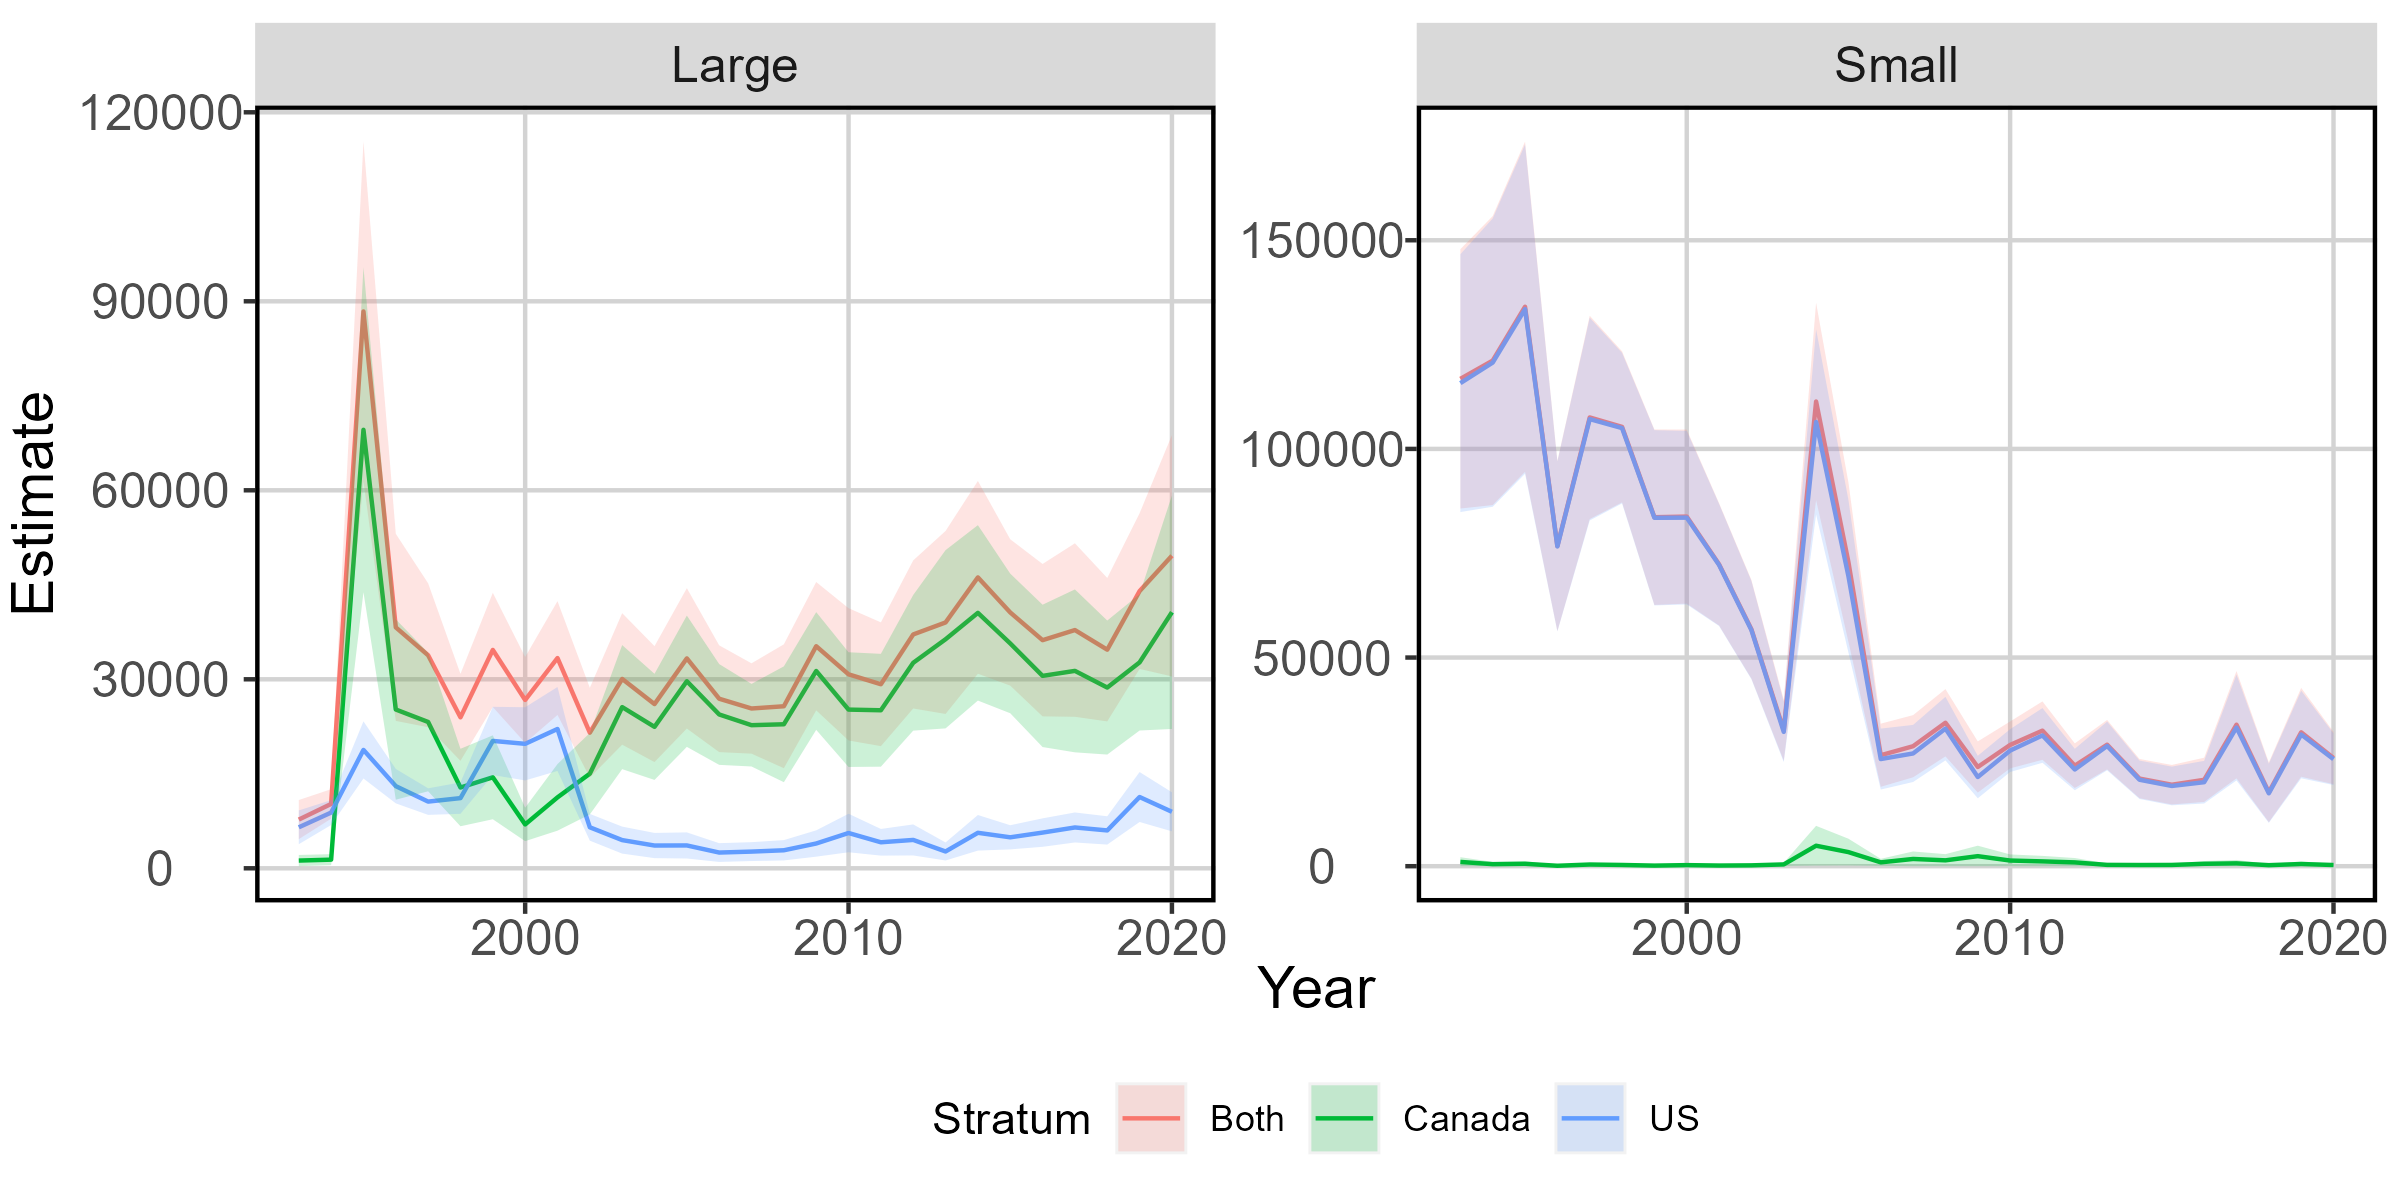
\includegraphics{C:/Users/klankowicz/Documents/GitHub/Atlantic-Bluefin-Tuna-Climate-Informed-Stock-Assessment/Plot_Output/index.png}
\caption{Fig. 4: Joint indices of abundance}
\end{figure}

\hypertarget{maps-of-spatial-density}{%
\subsection{Maps of spatial density}\label{maps-of-spatial-density}}

\begin{figure}
\centering
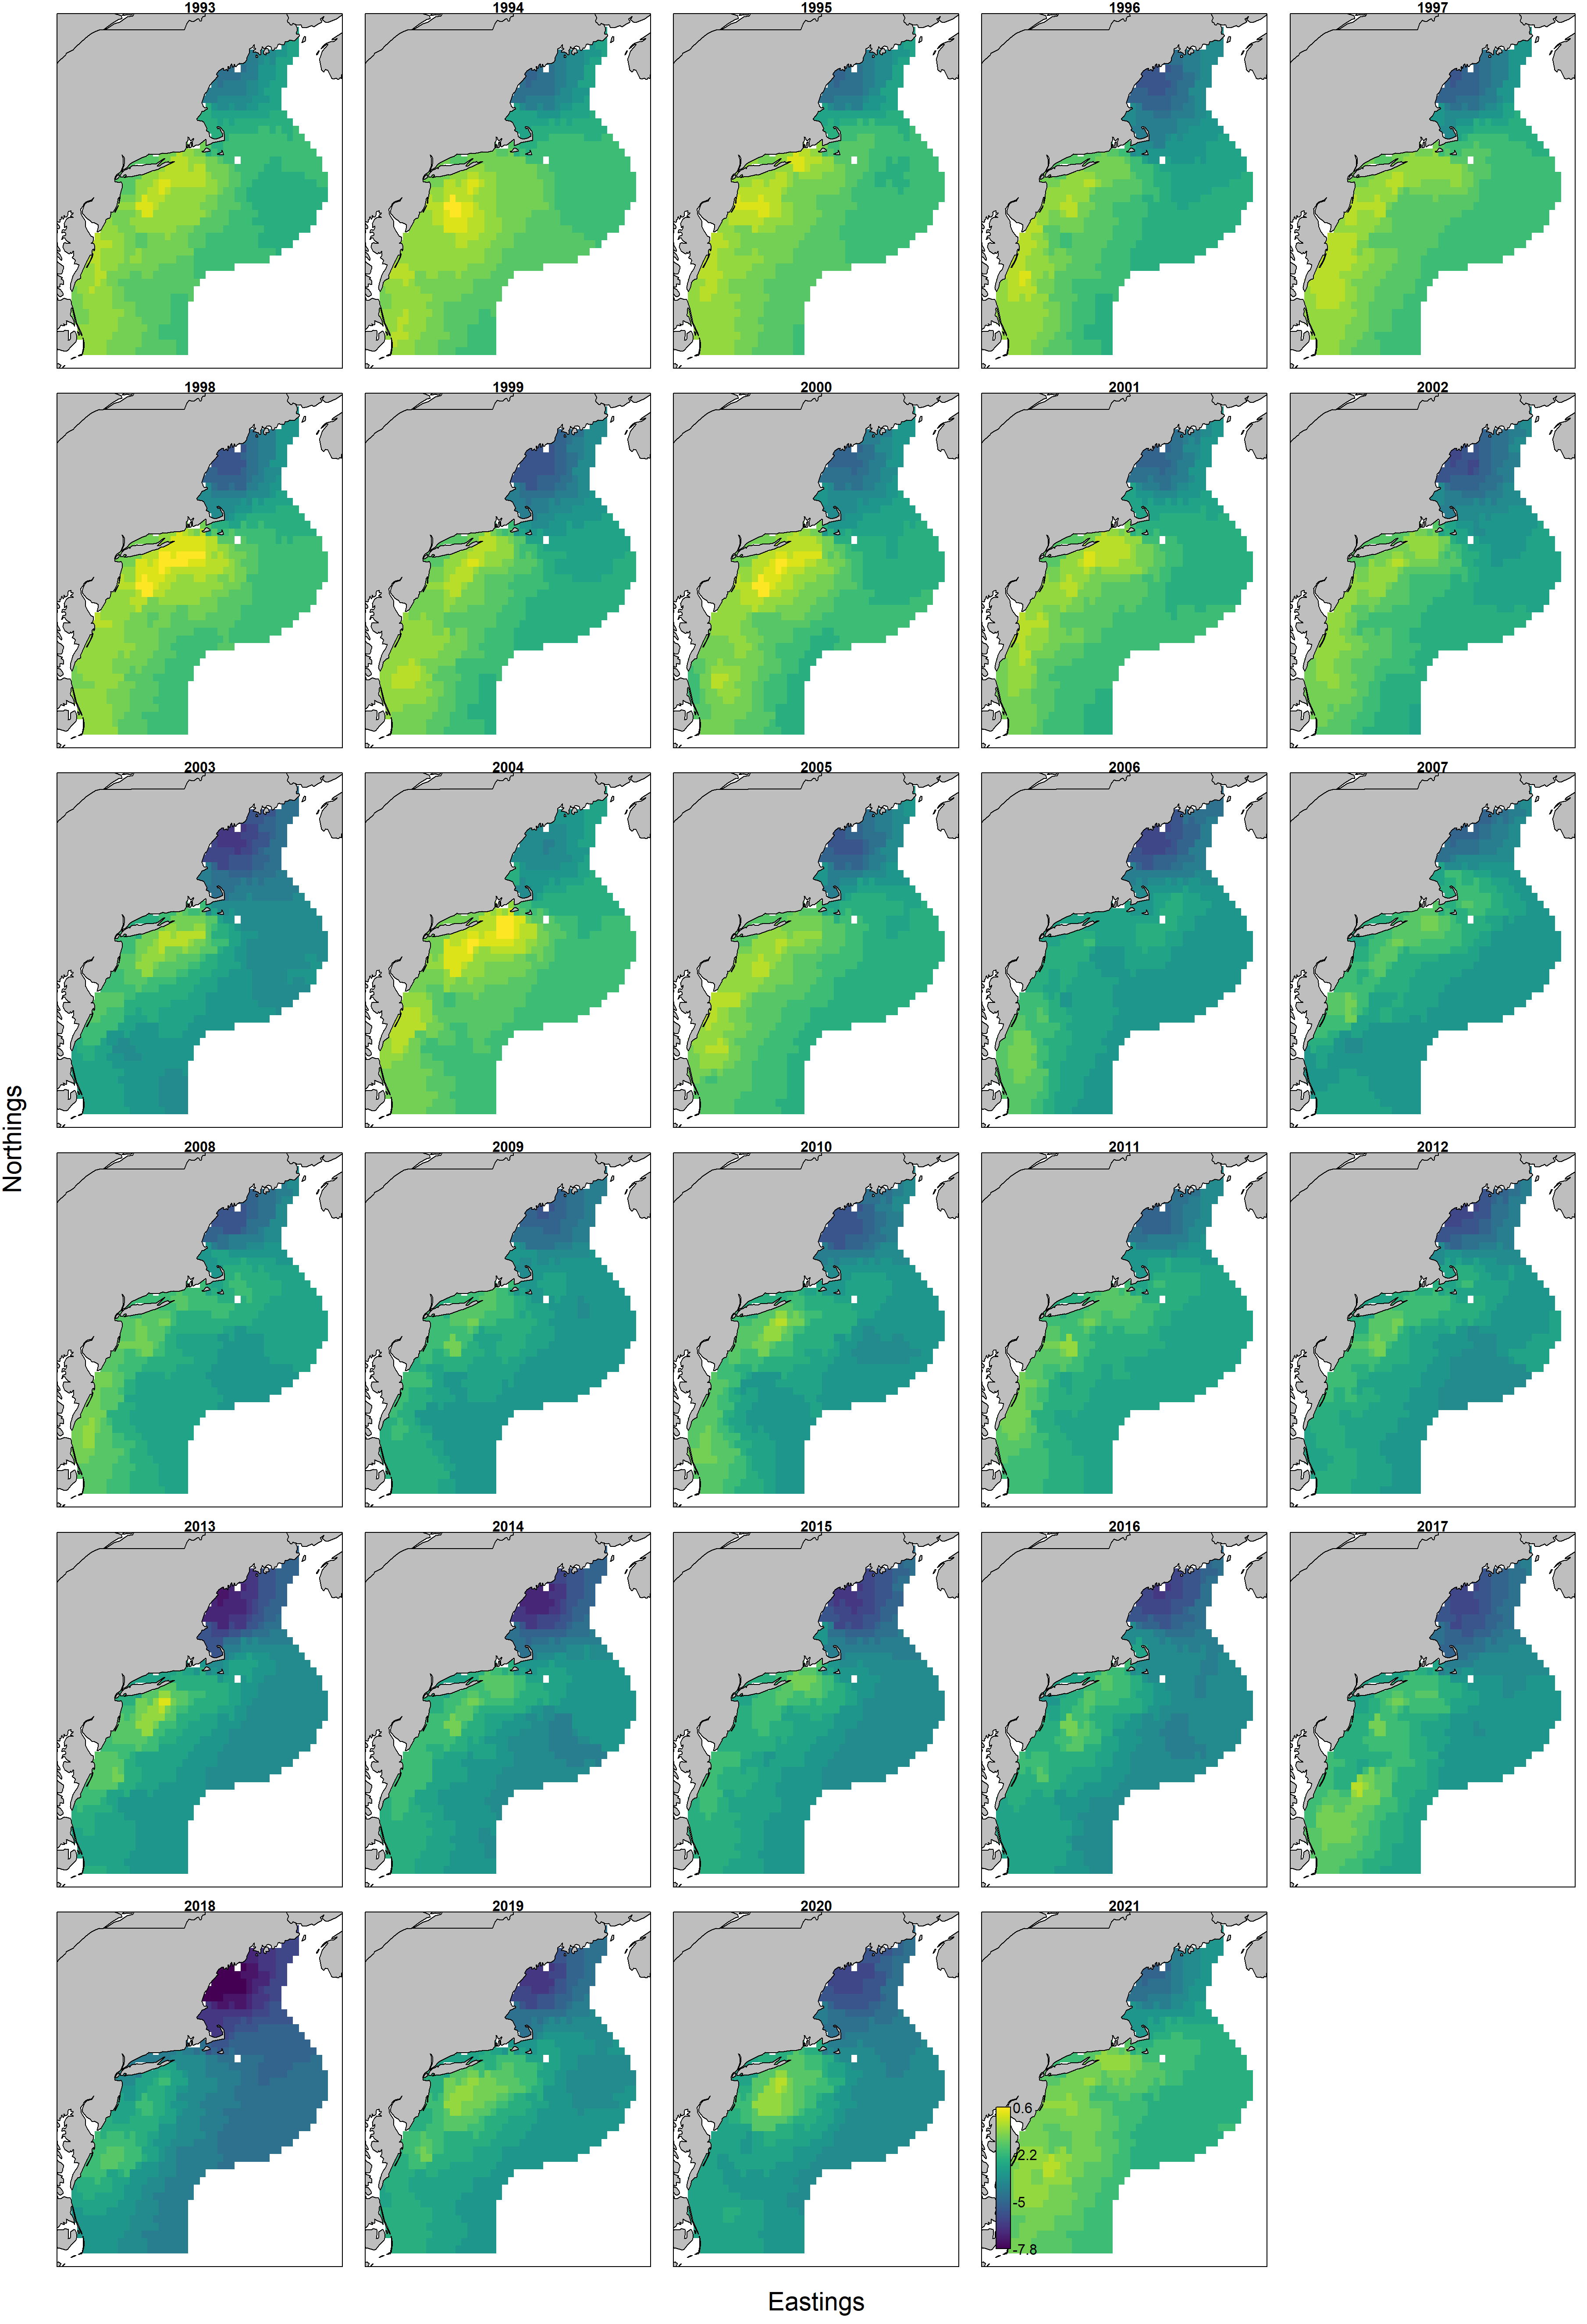
\includegraphics{C:/Users/klankowicz/Documents/GitHub/Atlantic-Bluefin-Tuna-Climate-Informed-Stock-Assessment/VAST_runs/tuna8/ln_density--Small-predicted.png}
\caption{Fig. 5:Small cod spatio-temporal density}
\end{figure}

\begin{figure}
\centering
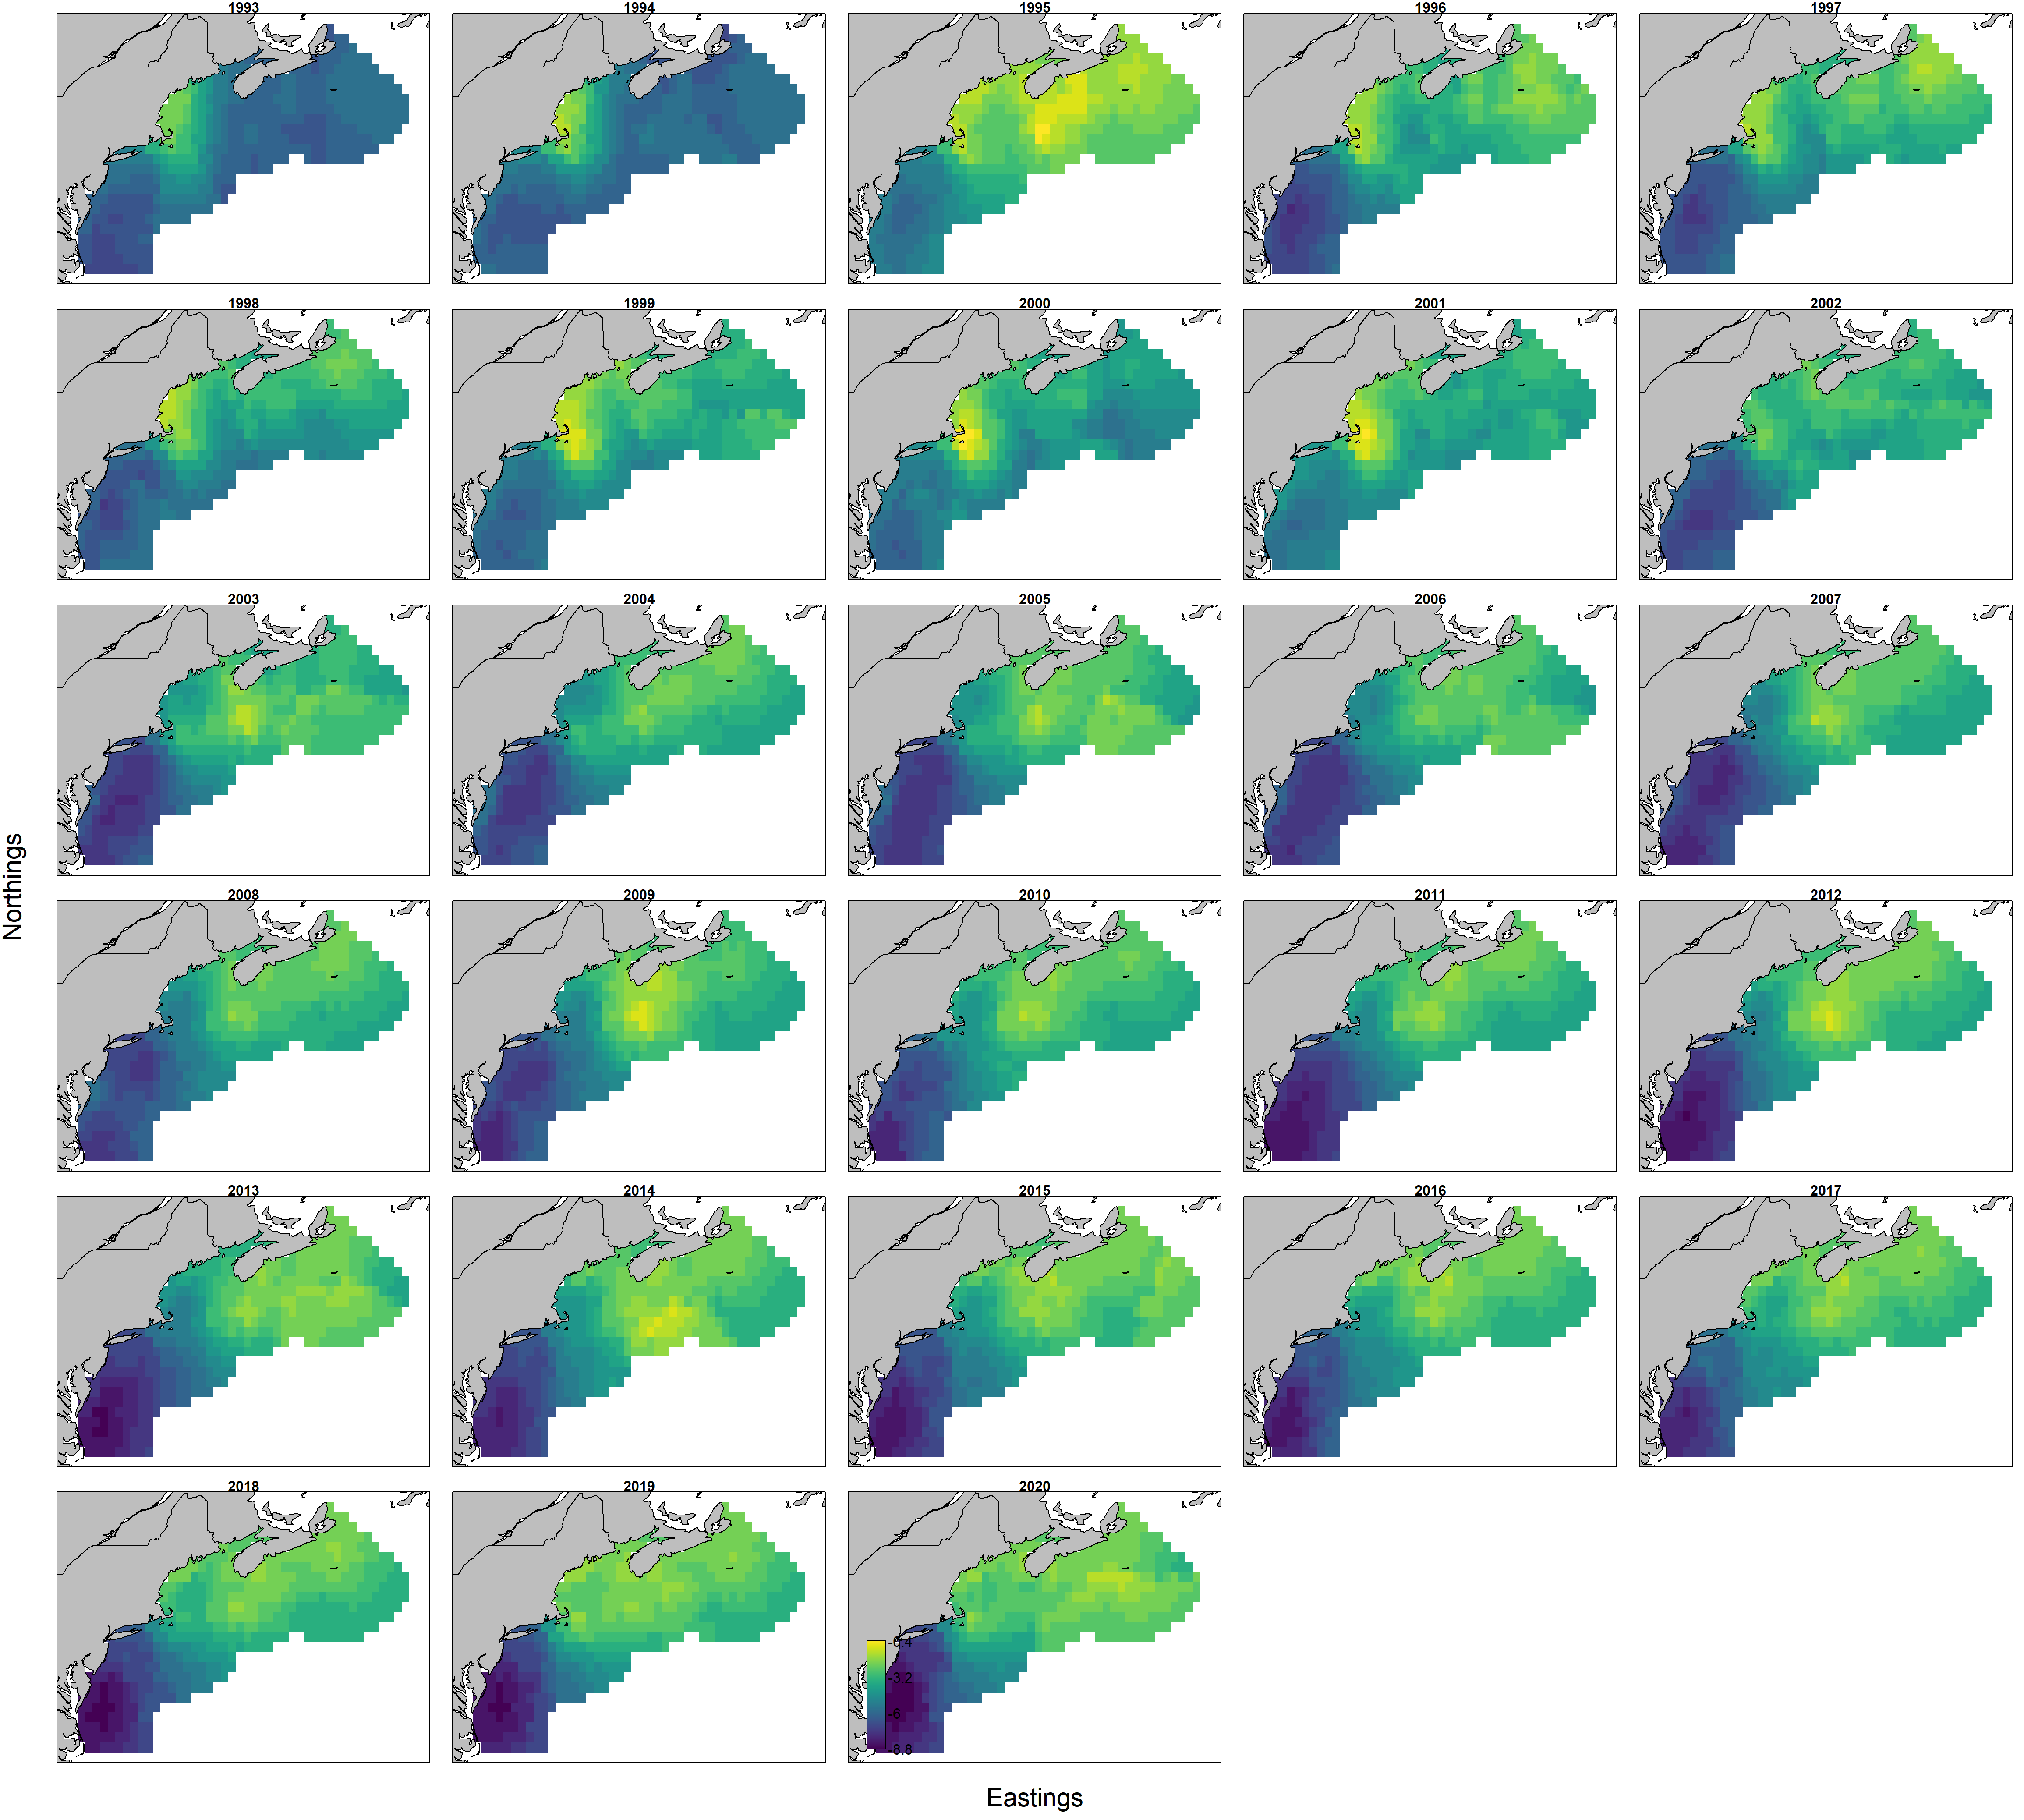
\includegraphics{C:/Users/klankowicz/Documents/GitHub/Atlantic-Bluefin-Tuna-Climate-Informed-Stock-Assessment/VAST_runs/tuna8/ln_density--Large-predicted.png}
\caption{Fig. 6: Large cod spatio-temporal density}
\end{figure}

\hypertarget{spatial-metrics-and-range-shifts}{%
\subsection{Spatial metrics and range shifts}\label{spatial-metrics-and-range-shifts}}

The model needs to be run once for each spatial strata in order to generate spatial metrics for each strata. As of right now, it takes approximately 9 hours to run on a laptop. Spatial metrics have only been generated for the Canadian stock.

\begin{figure}
\centering
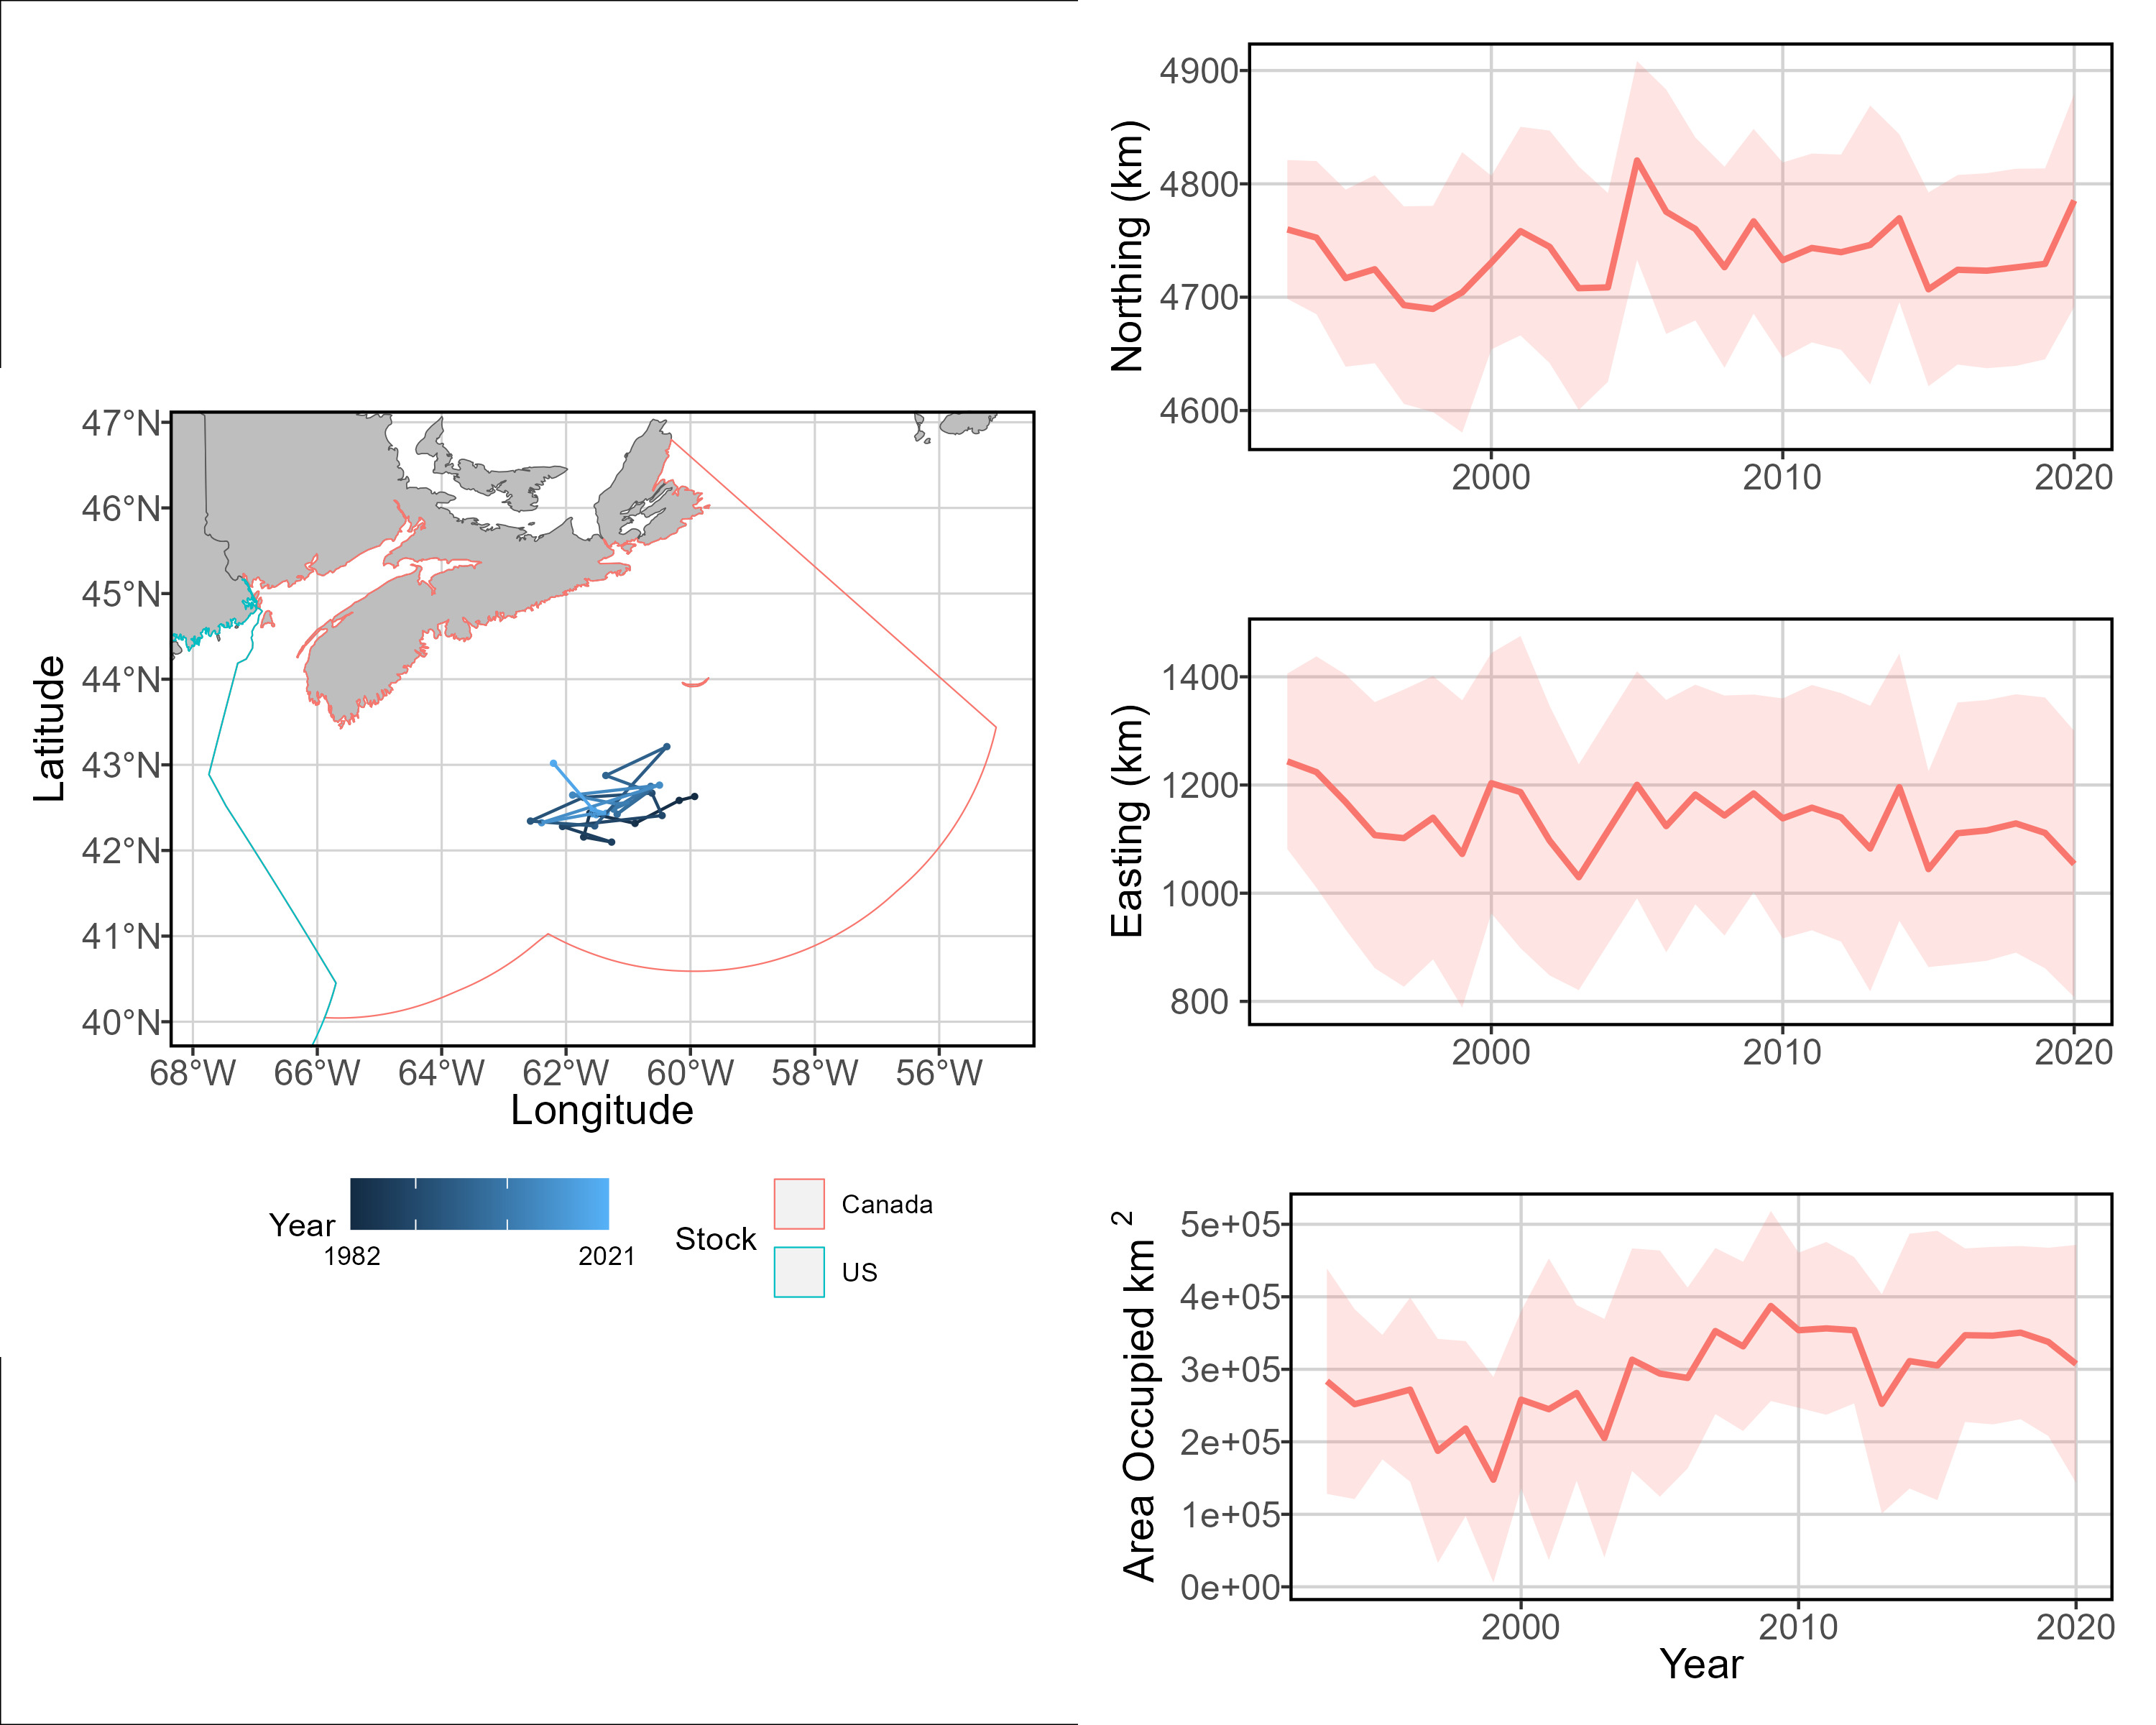
\includegraphics{C:/Users/klankowicz/Documents/GitHub/Atlantic-Bluefin-Tuna-Climate-Informed-Stock-Assessment/Plot_Output/location.info.Small.spring.Canada.png}
\caption{Fig. 7: Spatial metrics for small BFT in Canadian EEZ}
\end{figure}

\begin{figure}
\centering
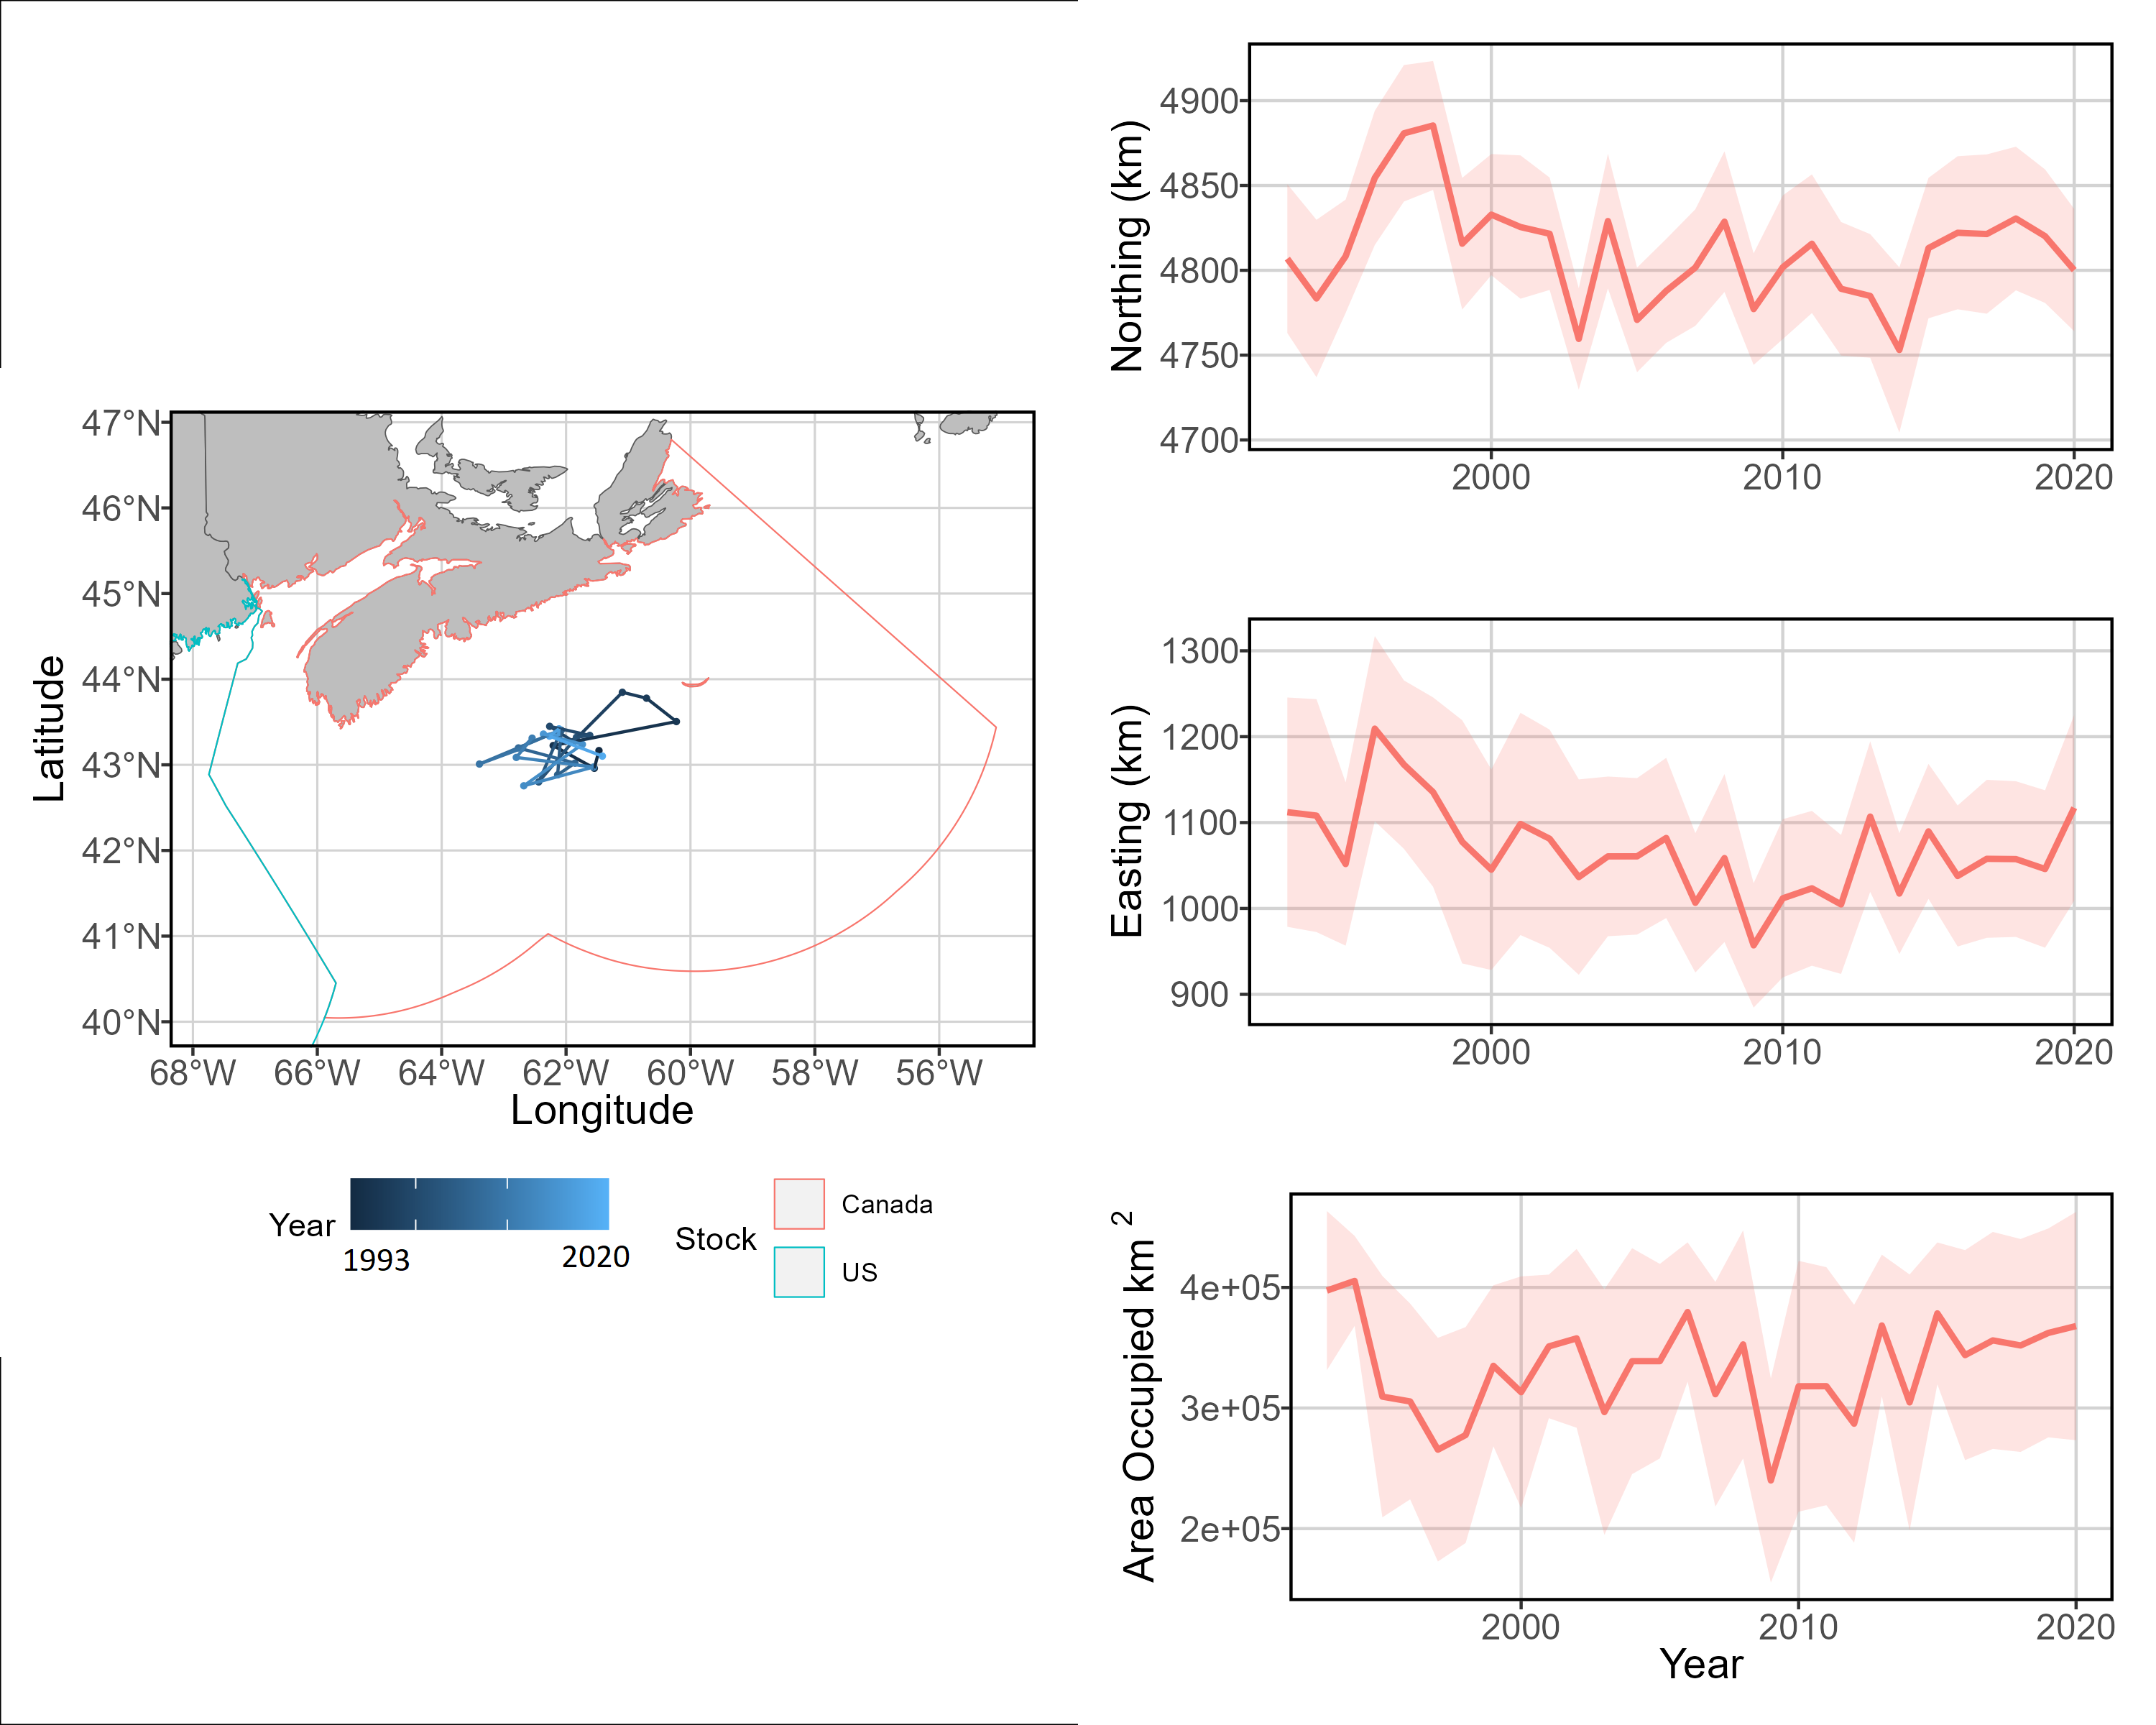
\includegraphics{C:/Users/klankowicz/Documents/GitHub/Atlantic-Bluefin-Tuna-Climate-Informed-Stock-Assessment/Plot_Output/location.info.Large.spring.Canada.png}
\caption{Fig. 8: Spatial metrics for large BFT in Canadian EEZ}
\end{figure}

It is interesting that the center of gravity for the small BFT stock in Canadian waters is typically further offshore than the large BFT stock. This is likely caused by the limited number of small BFT found in the Canadian EEZ and does not accurately reflect the true center of gravity for small BFT.

\hypertarget{model-caveats}{%
\section{Model caveats}\label{model-caveats}}

Both the American and Canadian datasets report very few sampling events with 0 catch. In the American dataset, the 1993-2002 period has no zeros reported. This likely skews the American indices to incorrectly report high BFT abundance in this period, despite the AR1 temporal correlation process.

The clear age-based spatial structure of BFT (smaller BFT prefer warmer southerly waters, larger BFT prefer colder northerly waters) likely causes issues in the generation of abundance indices. For example, the lack of small BFT in Canadian waters results in very little information for the model to predict and interpolate small BFT abundance in this area.

\hypertarget{refs}{}
\begin{CSLReferences}{1}{0}
\leavevmode\vadjust pre{\hypertarget{ref-thorson_2019}{}}%
Thorson, J. T. 2019. \href{https://doi.org/10.1016/j.fishres.2018.10.013}{Guidance for decisions using the {Vector} {Autoregressive} {Spatio}-{Temporal} ({VAST}) package in stock, ecosystem, habitat and climate assessments}. Fisheries Research 210:143--161.

\leavevmode\vadjust pre{\hypertarget{ref-thorson_comparing_2017}{}}%
Thorson, J. T., and L. A. K. Barnett. 2017. \href{https://doi.org/10.1093/icesjms/fsw193}{Comparing estimates of abundance trends and distribution shifts using single- and multispecies models of fishes and biogenic habitat}. ICES Journal of Marine Science 74(5):1311--1321.

\leavevmode\vadjust pre{\hypertarget{ref-thorson_accounting_2017}{}}%
Thorson, J. T., R. Fonner, M. A. Haltuch, K. Ono, and H. Winker. 2017. \href{https://doi.org/10.1139/cjfas-2015-0598}{Accounting for spatiotemporal variation and fisher targeting when estimating abundance from multispecies fishery data}. Canadian Journal of Fisheries and Aquatic Sciences 74(11):1794--1807.

\leavevmode\vadjust pre{\hypertarget{ref-thorson_2015}{}}%
Thorson, J. T., H. J. Skaug, K. Kristensen, A. O. Shelton, E. J. Ward, J. H. Harms, and J. A. Benante. 2015. \href{https://doi.org/10.1890/14-0739.1}{The importance of spatial models for estimating the strength of density dependence}. Ecology 96(5):1202--1212.

\end{CSLReferences}

\end{document}
